% Sim-to-Real Validity of Persona-Based Marketing-Copy Simulation
% arXiv preprint version — same template as doesitdefend/research/papers (article, twocolumn).
\documentclass[twocolumn]{article}

\usepackage{graphicx}
\usepackage{tikz}
\usetikzlibrary{arrows, positioning, arrows.meta, fit, backgrounds, calc}
\usepackage{booktabs}
\usepackage{amssymb}
\usepackage{amsmath}
\usepackage[breaklinks=true]{hyperref}
\usepackage{xurl}
\usepackage[numbers]{natbib}
\usepackage{microtype}
\usepackage{geometry}
\usepackage{xcolor}
\usepackage{xspace}
\usepackage{stfloats}
\usepackage{float}
\usepackage{caption}
\usepackage{enumitem}

\geometry{margin=1in}
\emergencystretch=2em  % absorb minor overfull boxes from long \texttt model ids

% Forbid hyphenation of cross-reference proper nouns and long identifiers, so they
% never split across the column edge (the doesitdefend margin-overflow convention).
\hyphenation{Section Sections Table Tables Figure Figures Appendix Appendices
  Equation Equations Upworthy Gemini Kendall Spearman Pew CoMPosT LOLA}

% Numbers come ONLY from variables.tex (auto-generated). Never hand-type a number.
% AUTO-GENERATED by scripts/generate_paper_variables.py — DO NOT EDIT BY HAND.
\newcommand{\nPackages}{399}
\newcommand{\nVariants}{1494}
\newcommand{\kendallTau}{0.084}
\newcommand{\kendallTauCILow}{0.020}
\newcommand{\kendallTauCIHigh}{0.147}
\newcommand{\spearmanRho}{0.104}
\newcommand{\spearmanRhoCILow}{0.035}
\newcommand{\spearmanRhoCIHigh}{0.172}
\newcommand{\topOneAcc}{34.6\%}
\newcommand{\topOneAccCILow}{29.8\%}
\newcommand{\topOneAccCIHigh}{39.1\%}
\newcommand{\randomTopOne}{30.4\%}
\newcommand{\bottomOneAcc}{37.1\%}
\newcommand{\bottomOneAccCILow}{32.3\%}
\newcommand{\bottomOneAccCIHigh}{41.9\%}
\newcommand{\reliableFraction}{23.5\%}
\newcommand{\sensNPackages}{1695}
\newcommand{\sensNVariants}{6978}
\newcommand{\sensKendallTau}{0.054}
\newcommand{\sensKendallTauCILow}{0.025}
\newcommand{\sensKendallTauCIHigh}{0.083}
\newcommand{\sensSpearmanRho}{0.069}
\newcommand{\baseTau}{0.361}
\newcommand{\baseTauCILow}{0.289}
\newcommand{\baseTauCIHigh}{0.430}
\newcommand{\baseRho}{0.350}
\newcommand{\baseTopOne}{49.2\%}
\newcommand{\baseTopOneCILow}{44.2\%}
\newcommand{\baseTopOneCIHigh}{54.3\%}
\newcommand{\hThreeN}{1678}
\newcommand{\hThreeTopOne}{0.059}
\newcommand{\hThreeTopOneCILow}{0.011}
\newcommand{\hThreeTopOneCIHigh}{0.107}
\newcommand{\baseSpreadSD}{0.054}
\newcommand{\personaSpreadSD}{0.054}
\newcommand{\nBaseRightPersonaWrong}{126}
\newcommand{\eaNPackages}{398}
\newcommand{\repGapMin}{0.28}
\newcommand{\repGapMax}{0.32}
\newcommand{\repNDatasets}{5}
\newcommand{\confNPackages}{1866}
\newcommand{\confPersonaTau}{0.070}
\newcommand{\confBaselineTau}{0.393}
\newcommand{\mindGap}{0.038}
\newcommand{\baseTieRate}{17.8\%}
\newcommand{\baseTopOneFair}{50.0\%}
\newcommand{\baseTopOneNonDegen}{52.9\%}
\newcommand{\stabTauSD}{0.025}
\newcommand{\stabTopOneSD}{0.008}
\newcommand{\xfModel}{gpt-4.1}
\newcommand{\xfN}{399}
\newcommand{\xfPairedN}{395}
\newcommand{\xfPersonaTau}{0.082}
\newcommand{\xfBaselineTau}{0.300}
\newcommand{\xfPersonaTop}{35.8\%}
\newcommand{\xfBaselineTop}{49.1\%}
\newcommand{\xfGapTau}{+0.214}
\newcommand{\xfGapTauCILow}{0.134}
\newcommand{\xfGapTauCIHigh}{0.296}
\newcommand{\xfGapTopPP}{+13.2}
\newcommand{\xfGapTopPPCILow}{6.6}
\newcommand{\xfGapTopPPCIHigh}{19.7}


\title{Do Synthetic Personas Predict Real Audience Response?\\
A Sim-to-Real Study Where a No-Persona Baseline\\
Beats Persona-Based Copy Simulation}

\author{Alexandre Cristov\~ao Maiorano\\
\texttt{alexandre@lumytics.com}}
\date{}

\begin{document}

\twocolumn[
  \begin{@twocolumnfalse}
    \maketitle
    % Abstract — every number is a macro from variables.tex (auto-generated). No raw digits.
\begin{abstract}
Marketers increasingly use large language models (LLMs) as ``synthetic personas'' to predict how
an audience will react to a piece of copy before it ships, encouraged by evidence that
profile-conditioned LLMs can mimic human samples~\citep{argyleSiliconSampling}. But is that
prediction actually valid against real behaviour---and does the persona machinery help? We present
a sim-to-real validity study using the Upworthy Research Archive~\citep{matiasUpworthy}---thousands
of headline A/B tests in which real readers were shown competing variants and their clicks
recorded---as held-out ground truth. We compare a ten-persona panel, grounded in the real
audience's demographics~\citep{holcomb2013newsuse}, against a no-persona zero-shot baseline that
simply asks the model how likely a typical reader is to click. Two findings stand out. First,
\textbf{ground-truth reliability is the binding constraint}: most A/B tests have no statistically
distinguishable winner~\citep{kohavi2009controlled}, so validity can only be measured on the
reliable subset ($n=\nPackages{}$). Second, and counter to the persona-simulation premise,
\textbf{persona conditioning degrades predictive validity}: the no-persona baseline ranks variants
markedly better (Kendall $\tau=\baseTau{}$, a medium effect; top-1 accuracy \baseTopOne{}) than the
persona panel ($\tau=\kendallTau{}$; top-1 \topOneAcc{}), with non-overlapping confidence
intervals. Asking the model directly taps an accurate population-level prior on what gets clicked,
whereas forcing it to role-play specific personas injects bias and noise. The result replicates
across three independent Upworthy splits and holds in direction on a different-domain, more-recent
news dataset, and is robust to seed, prompt phrasing, and model choice---it holds across three
Gemini tiers and reproduces on a different model family (OpenAI gpt-4.1) with a significant paired
gap. The practical takeaway:
for predicting aggregate engagement, a plain LLM ranker beats persona simulation---synthetic
personas are not merely a weak predictor, they are worse than not using them. All numbers are
regenerated from a public, artifact-first replication package.
\end{abstract}

    \vspace{2mm}
  \end{@twocolumnfalse}
]

\section{Introduction}

Before launching a campaign, marketers want to know which version of a message will land. A fast-
growing practice replaces (or precedes) live A/B testing with \emph{synthetic audience
simulation}: a large language model (LLM) is conditioned on a set of audience ``personas'' and
asked to react to each candidate message, and the message its personas prefer is shipped. The
appeal is obvious---instant, cheap feedback---and it is encouraged by findings that
profile-conditioned LLMs can reproduce aspects of real human samples, an idea sometimes called
``silicon sampling''~\citep{argyleSiliconSampling}.

The appeal, however, outruns the evidence. The premise that a synthetic persona predicts how a
\emph{real} audience behaves is rarely tested against real outcomes, because doing so requires
ground truth that pairs concrete copy with measured audience response. We borrow the
\emph{sim-to-real} framing from robotics---how well does behaviour measured in simulation transfer
to the real world?---and instantiate it with the Upworthy Research
Archive~\citep{matiasUpworthy}: thousands of A/B tests (which we call \emph{packages}) in which
competing headline variants were shown to the same real traffic and their click-through rates
recorded. This lets us ask, for held-out copy never seen during persona design, whether the
simulator orders the variants the way the audience did.

We report two main findings. First, the dominant obstacle is not the model but the data: in most
A/B tests the real winner is not statistically distinguishable from the runner-up, so no predictor
can recover it---validity is only meaningful on the reliable subset. Second, and contrary to the
premise of persona simulation, \emph{persona conditioning hurts}: a no-persona zero-shot baseline
that simply asks the model how likely a typical reader is to click ranks the variants markedly
better (a medium effect) than the demographically grounded ten-persona panel (a small,
barely-significant effect), with non-overlapping confidence intervals. The base model holds an
accurate population-level prior on clickability; forcing it to role-play specific personas pulls
it away from that prior. We pre-register effect-size thresholds and report seed-stability and a
model comparison so neither effect is overstated.

\paragraph{Contributions.}
\begin{enumerate}[leftmargin=*]
  \item A reproducible \emph{sim-to-real} validity protocol for copy simulation, using a public,
        held-out A/B-tested benchmark~\citep{matiasUpworthy} as ground truth.
  \item A ground-truth-reliability filtering step (significant-winner A/B tests) that prevents
        validating a predictor against statistical noise~\citep{kohavi2009controlled}.
  \item A within-package ranking evaluation with a construct-matched click-intent elicitation,
        a no-persona zero-shot baseline that isolates the value of persona conditioning,
        pre-registered effect-size thresholds~\citep{cohen1988power}, bootstrap CIs, seed-stability,
        and a cost/quality model comparison.
  \item An artifact-first replication package: every reported number is regenerated from
        aggregated artifacts by public scripts.
\end{enumerate}

\paragraph{Research questions.}
\begin{description}[leftmargin=*]
  \item[RQ1] Do the personas' predicted ranking match the real click-through ranking on copy with
        a reliable winner, and do they beat a no-persona zero-shot baseline?
  \item[RQ2] Does predictive validity increase with the strength of the real effect?
  \item[RQ3] Is the result robust to the intent-vs-engagement construct gap, to seed sampling,
        and to model choice?
\end{description}

\section{Related Work}

\paragraph{LLMs as proxies for human populations.}
A growing body of work uses language models conditioned on demographic or attitudinal profiles
to approximate human samples---``silicon sampling''~\citep{argyleSiliconSampling}---and surveys
the promise and limits of LLMs as tools for computational social science~\citep{ziems2024css}.
The evidence, however, is mixed. On the supportive side, profile-conditioned models can reproduce
aggregate survey \emph{distributions}~\citep{argyleSiliconSampling}, and agents grounded in a
two-hour interview \emph{per person} replicate that individual's survey responses at $\approx$85\% of
the person's own two-week test--retest reliability~\citep{park2024agents}---though both successes are
on \emph{stated attitudes}, and the latter buys its fidelity with rich per-person grounding rather
than the cheap demographic profile we test. On the cautionary side,
LLM ``survey responses'' latch onto spurious option ordering rather than
meaning~\citep{dominguezolmedo2024questioning}; persona variables explain less than 10\% of the
variance in subjective annotation and help only when the persona--outcome correlation is
strong~\citep{hu2024persona}; assigning personas can surface biases and \emph{degrade}
performance on objective tasks~\citep{zheng2024helpful}; and persona simulations tend toward
\emph{caricature}~\citep{cheng2023compost}; and ad-hoc persona \emph{generation} itself injects
systematic bias, with election and survey forecasts deviating from real
outcomes~\citep{li2025personacatch}. Our work contributes a direct sim-to-real
\emph{validity} test against measured real-world behaviour (not survey distributions), and—unlike
prior work focused on accuracy or annotation—isolates the marginal effect of persona conditioning
with a no-persona baseline on a copy-ranking task.

\paragraph{The Upworthy archive and headline performance.}
The Upworthy Research Archive~\citep{matiasUpworthy} has supported large-scale analyses of what
makes headlines succeed; for example, negativity in headlines increases consumption at
scale~\citep{robertson2023negativity}. These works model \emph{aggregate} drivers of clicks; we
instead use the archive as a held-out benchmark to test whether an external persona-based
simulator can \emph{predict} the within-test winner. Most directly, concurrent work on the same
archive~\citep{ye2024lola} reports that pure-LLM headline prediction (prompting, embeddings,
fine-tuning) only marginally beats random; our results refine this picture by showing that
\emph{after} filtering to A/B tests with a reliable winner, a no-persona LLM ranker is in fact a
medium-strength predictor---and that adding personas erases this. The finding that personas can
introduce harmful bias echoes work on LLM simulations producing
\emph{caricatures}~\citep{cheng2023compost}.

\paragraph{Construct validity and effect sizes.}
We frame the intent-vs-engagement mismatch using the classical construct-validity
framework~\citep{cronbach1955construct} and pre-register effect-size thresholds following
Cohen~\citep{cohen1988power}.

\section{Sim-to-Real Validity Framework}
\label{sec:framework}

\paragraph{Setup.}
Figure~\ref{fig:protocol} summarises the protocol. A \emph{package} is an A/B test containing two
or more copy \emph{variants} shown to the same real audience; each variant $v$ has an observed
click-through rate $\mathrm{CTR}(v)$ and a simulator-predicted score $\texttt{pred\_score}(v)$
(Section~\ref{sec:system}).
% Sim-to-real protocol diagram (self-contained TikZ; no external data).
% figure* spans both columns; resizebox keeps the horizontal pipeline within \textwidth.
\begin{figure*}[t]
  \centering
  \resizebox{0.92\textwidth}{!}{%
  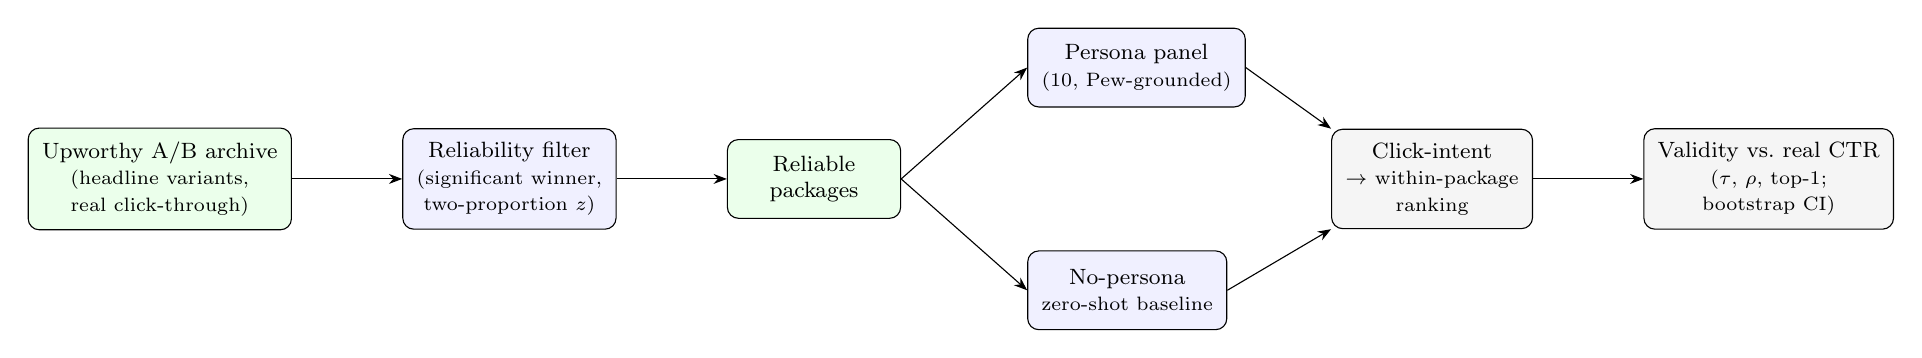
\begin{tikzpicture}[
    font=\footnotesize,
    box/.style={draw, rounded corners, align=center, inner sep=5pt, minimum height=10mm, minimum width=22mm},
    data/.style={box, fill=green!8},
    proc/.style={box, fill=blue!6},
    res/.style={box, fill=gray!8},
    >=Stealth, node distance=8mm and 14mm,
  ]
    \node[data] (arch) {Upworthy A/B archive\\\scriptsize(headline variants,\\\scriptsize real click-through)};
    \node[proc, right=of arch] (filt) {Reliability filter\\\scriptsize(significant winner,\\\scriptsize two-proportion $z$)};
    \node[data, right=of filt] (rel) {Reliable\\packages};
    \node[proc, above right=4mm and 16mm of rel] (panel) {Persona panel\\\scriptsize(10, Pew-grounded)};
    \node[proc, below right=4mm and 16mm of rel] (base) {No-persona\\\scriptsize zero-shot baseline};
    \coordinate (fork) at ($(panel.east)!0.5!(base.east)$);
    \node[res, right=12mm of fork, anchor=west] (score) {Click-intent\\\scriptsize$\to$ within-package\\\scriptsize ranking};
    \node[res, right=of score] (val) {Validity vs.\ real CTR\\\scriptsize($\tau$, $\rho$, top-1;\\\scriptsize bootstrap CI)};

    \draw[->] (arch) -- (filt);
    \draw[->] (filt) -- (rel);
    \draw[->] (rel.east) -- (panel.west);
    \draw[->] (rel.east) -- (base.west);
    \draw[->] (panel.east) -- (score.north west);
    \draw[->] (base.east) -- (score.south west);
    \draw[->] (score) -- (val);
  \end{tikzpicture}%
  }
  \caption{The sim-to-real validity protocol. Real A/B tests are filtered to those with a
  statistically reliable winner; the persona panel and a no-persona baseline each score the
  variants, which are ranked within each package and compared to the real click-through ordering.}
  \label{fig:protocol}
\end{figure*}
 Because variants
within a package share an audience, the package defines a controlled comparison.

\paragraph{Why ranking, not absolute CTR.}
We evaluate \emph{within-package ranking} rather than absolute CTR for two reasons. First, CTR
levels vary across packages for reasons unrelated to copy (topic, timing, audience), so only the
within-package contrast is attributable to the copy. Second, the simulator's score and the
benchmark outcome are different constructs (intent vs.\ engagement; Section~\ref{sec:discussion}),
so a ranking criterion is robust to scale and calibration differences. Concretely, a useful
copy simulator need not predict the CTR number---it needs to order candidate variants the way
the real audience does.

\paragraph{Metrics.}
For each package we compare the CTR ordering and the \texttt{pred\_score} ordering with: top-1
winner accuracy (did the predicted best variant match the real best), Kendall's
$\tau$~\citep{kendall1938}, and Spearman's $\rho$~\citep{spearman1904}. Package-level values are
aggregated across packages with bootstrap confidence intervals (Section~\ref{sec:setup}).

\section{Method Under Test}
\label{sec:system}

We evaluate persona-based copy simulation as a \emph{method}, instantiated as a controlled
research harness rather than any specific deployed product: given a piece of copy and an audience,
the harness instantiates a panel of synthetic personas and elicits each persona's reaction, then
aggregates these into a ranking. We make the instantiation fully explicit (personas, prompt, and
aggregation below) so the result is attributable to the technique, not to an opaque product
configuration. The harness and all its inputs are released in the replication package.

\paragraph{Persona panel.}
The panel is a fixed, versioned set of $P=10$ personas (Appendix~\ref{sec:appendix}). To avoid
authoring bias, the personas are authored from public demographics rather than reused from any
product; they are constructed to represent the real Upworthy-era audience---U.S.\ social-media news consumers
circa 2013--2015---using the demographic structure reported by Pew
Research~\citep{holcomb2013newsuse} (age, gender, and platform mix, e.g.\ Facebook news
consumers skewing female and Twitter news consumers skewing younger). Each persona is a short
natural-language profile (age band, gender, primary platform, news-engagement level, and a
behavioural description).

\paragraph{Elicitation and the predicted score.}
For each headline variant and each persona we query an instruction-tuned LLM
(\texttt{gemini-3.1-flash-lite}; selected by the model comparison in Section~\ref{sec:setup}),
conditioning on the persona profile and asking, in the persona's voice, how likely they are to
click the headline. The model returns a structured \texttt{click\_intent} value in $[0,1]$.

Crucially, the \textbf{predicted score} we evaluate is this \emph{click-intent}, aggregated by the
\textbf{arithmetic mean} over the panel (and over Monte~Carlo draws):
\[
\texttt{pred\_score}(v) \;=\; \frac{1}{P D}\sum_{i=1}^{P}\sum_{d=1}^{D} \texttt{click\_intent}_{i,d}(v).
\]
We use the simple mean for interpretability; alternative aggregations (median, rank fusion) are a
sensitivity dimension we leave to future work (Section~\ref{sec:discussion}). We elicit
click-intent directly because the benchmark outcome is click-through (engagement); the construct
alignment and its limits are analysed in Section~\ref{sec:discussion}. Within a package, variants
are ranked by \texttt{pred\_score}; the no-persona baseline (Section~\ref{sec:setup}) uses the
identical scoring and aggregation with a single generic reader and no demographic conditioning.

\paragraph{Sampling and reproducibility.}
Generation uses temperature $0.8$ (the simulator's robust-sampling setting) with a fixed seed
forwarded to the model; each Monte~Carlo draw uses a distinct seed, and every prediction record
stores the model id, seed, temperature, draw count, and panel size for provenance. The reported
primary estimate averages $D{=}3$ draws per persona to control seed-level sampling noise
(Section~\ref{sec:setup}).

\section{Experimental Setup}
\label{sec:setup}

\paragraph{Corpus.}
We use the exploratory split of the Upworthy Research Archive~\citep{matiasUpworthy}. Rows are
grouped into packages (A/B tests) by test id; within a package we aggregate impressions and
clicks per \emph{distinct headline}, since variants that differ only by image cannot be
distinguished by a text-only simulator. We keep packages with $\geq 2$ distinct headlines and
$\geq 3{,}000$ impressions per headline-variant, the latter for click-through reliability in
online controlled experiments~\citep{kohavi2009controlled}. This yields \sensNVariants{} eligible
variants across \sensNPackages{} A/B tests; the corpus is locked with a content hash and never re-hosted.

\paragraph{Ground-truth reliability filtering.}
Within-package click-through differences are often tiny and statistically indistinguishable from
noise; validating a predictor against a noisy label is ill-posed. We therefore mark a package as
having a \emph{reliable winner} when its top-CTR headline significantly beats the runner-up by a
one-sided two-proportion $z$-test ($p<0.05$). The \textbf{primary analysis} uses the
reliable-winner packages ($n=\nPackages{}$); a \textbf{sensitivity analysis} reports all
predicted packages. This filters on ground-truth reliability, \emph{not} on effect direction, so
it does not bias the validity estimate.

\paragraph{Metrics.}
Ranking agreement is measured \emph{within} each package by top-1 winner accuracy, Kendall's
$\tau$~\citep{kendall1938}, and Spearman's $\rho$~\citep{spearman1904}, aggregated across
packages with $95\%$ percentile bootstrap confidence intervals ($10{,}000$ resamples over
packages, seed $42$)~\citep{efron1979bootstrap}. The top-1 baseline is the expected accuracy of
random guessing given each package's variant count. We additionally report a decision-relevant
metric---the \emph{fraction of achievable CTR lift captured} by the top-1 pick (0 = picks the
worst variant, 1 = the real best)---since a copy tool is ultimately judged by the click-through it
secures, not only by rank correlation.

\paragraph{Replication and robustness.}
Beyond the primary (exploratory) split we replicate on two further independent Upworthy splits
(holdout, confirmatory) and on two further platforms/domains: MIND news (2019, grouped by
subcategory) and Reddit title reposts (2008--12, same image and subreddit, different titles). The
same reliable-winner filter (one-sided two-proportion $z$-test on the per-variant outcome rate) is
applied to every dataset---click-through for Upworthy and MIND, upvote ratio for Reddit. We also
probe prompt sensitivity with a third-person persona framing and a reworded baseline.

\paragraph{Power and effect-size thresholds.}
Following Cohen~\citep{cohen1988power}, we pre-register $\tau,\rho \geq 0.10$ (with a CI excluding
zero) as the bar for a meaningful effect. A power analysis ($\alpha{=}0.05$, power$=0.80$) gives
the required package counts: $n{=}347$ to detect $\rho{=}0.15$ and $n{=}663$ to detect the
observed top-1 margin. Using all eligible packages supplies $n=\nPackages{}$ reliable packages,
which powers the rank-correlation claim around $\rho{\approx}0.15$; we therefore report top-1
accuracy as an under-powered secondary outcome rather than over-claiming.

\paragraph{No-persona baseline.}
To isolate the marginal value of persona conditioning, we run a baseline that removes the
demographic disaggregation: a single generic ``typical U.S.\ social-media news reader in 2014''
prompt with no demographic profile---equivalently, one \emph{aggregate} (population-level)
persona---scored and aggregated identically to the panel. For a fair comparison it
receives the same per-variant query budget as the panel ($P{\times}D=30$ samples per variant, here
as $30$ draws of the single prompt).

\paragraph{Model selection.}
A pilot compared \texttt{gemini-3.1-flash-lite}, \texttt{gemini-2.5-flash}, and
\texttt{gemini-3.5-flash} on a common subset; their validity confidence intervals were mutually
overlapping (statistically indistinguishable), so we select the cheapest and fastest,
\texttt{gemini-3.1-flash-lite}, for the full study.

\paragraph{Reproducibility and replication.}
All randomness is seeded (corpus sampling, bootstrap, and LLM generation; seeds in
Appendix~\ref{sec:appendix}). The primary estimate averages $D{=}3$ Monte~Carlo draws (distinct
seeds) per persona, because a seed-stability check showed single-seed rank estimates vary by
$\approx \stabTauSD{}$ in $\tau$---non-trivial relative to the effect size; the
sensitivity-only (non-reliable) packages use a single draw. Predictions are written
incrementally to a per-observation checkpoint, making runs crash-safe and resumable.

\section{Results}
\label{sec:results}

\paragraph{Ground-truth reliability is the binding constraint.}
Of the \sensNPackages{} eligible packages, only \nPackages{} (\reliableFraction{}) have a
statistically reliable within-package winner (Figure~\ref{fig:reliability}).

\begin{figure}[t]
  \centering
  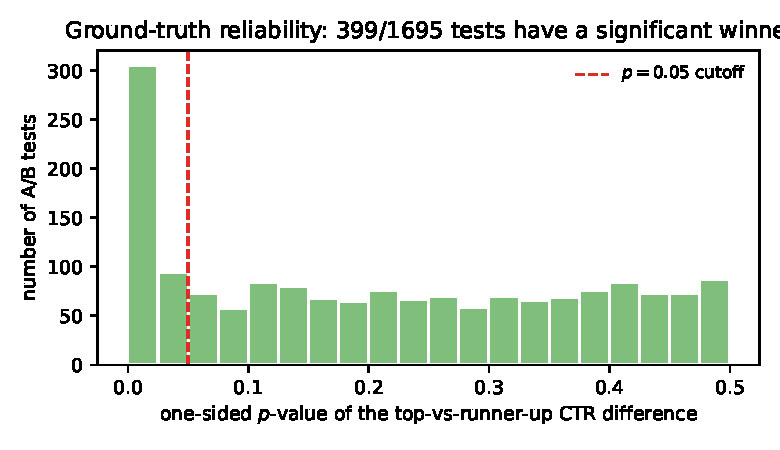
\includegraphics[width=0.92\linewidth]{figures/reliability.pdf}
  \caption{Distribution of the one-sided $p$-value for the top-vs-runner-up CTR difference across
  the eligible A/B tests. Only the tests to the left of the dashed cutoff have a statistically
  reliable winner; the rest cannot be predicted by construction.}
  \label{fig:reliability}
\end{figure} In the remainder the real click-through difference is indistinguishable
from noise, so no predictor can recover the ordering by construction. The primary analysis is
therefore restricted to the \nPackages{} reliable packages.

\paragraph{Personas vs.\ a no-persona baseline (RQ1).}
Table~\ref{tab:validity} reports within-package ranking agreement (Section~\ref{sec:framework})
on the reliable packages for both methods. The headline result is that \emph{persona conditioning
hurts}. The no-persona zero-shot baseline ranks variants well---Kendall $\tau=\baseTau{}$ (95\% CI
[\baseTauCILow{}, \baseTauCIHigh{}]), a medium effect by Cohen's
conventions~\citep{cohen1988power}, with top-1 accuracy \baseTopOne{} (95\% CI
[\baseTopOneCILow{}, \baseTopOneCIHigh{}]) against a random baseline of \randomTopOne{}. The
ten-persona panel is far weaker: $\tau=\kendallTau{}$ (95\% CI
[\kendallTauCILow{}, \kendallTauCIHigh{}]) and top-1 \topOneAcc{}, with confidence intervals that
do not overlap the baseline's on any metric (Figure~\ref{fig:comparison}). Persona conditioning
thus does not merely fail to help---it actively degrades a usable signal that the base model
already has.

\begin{figure}[t]
  \centering
  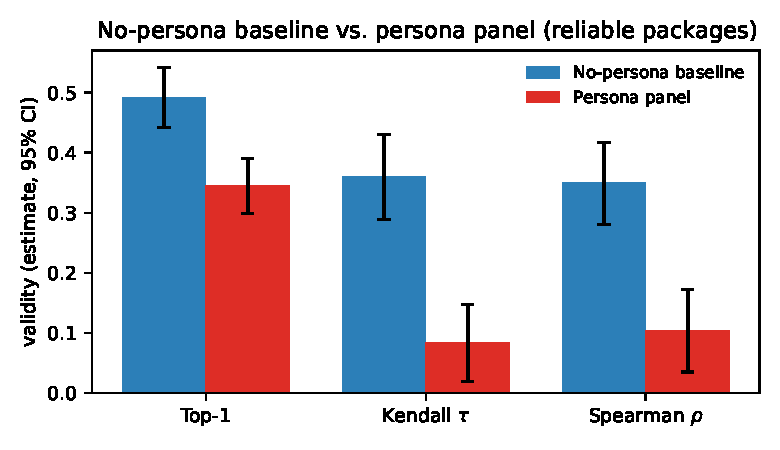
\includegraphics[width=0.92\linewidth]{figures/comparison.pdf}
  \caption{Headline result: the no-persona baseline outperforms the persona panel on every
  metric, with non-overlapping 95\% bootstrap CIs, on the reliable-winner packages.}
  \label{fig:comparison}
\end{figure}

\paragraph{The persona panel in isolation.}
Considered on its own, the panel's predictive validity is weak but statistically significant
($\tau$ and $\rho$ CIs exclude zero), at or below Cohen's small-effect threshold. Its top-1 CI
includes the random baseline, so it does not reliably pick the single best variant; it is, if
anything, slightly better at flagging the \emph{worst} variant (\bottomOneAcc{}) than the best
(\topOneAcc{}), detecting clearly weak copy more readily than winners.

% AUTO-GENERATED by scripts/generate_validity_table.py — DO NOT EDIT BY HAND.
\begin{table*}[t]
  \centering
  \caption{Headline result: a no-persona zero-shot ranker vs.\ the persona panel on the reliable-winner packages ($n=399$). The no-persona baseline is substantially better on every metric (non-overlapping CIs). Random top-1 baseline 30.4\%. 95\% bootstrap CIs.}
  \label{tab:validity}
  \small
  \begin{tabular}{lccc}
    \toprule
    Method & Top-1 [95\% CI] & Kendall $\tau$ [95\% CI] & Spearman $\rho$ [95\% CI] \\
    \midrule
    No-persona baseline & 49.2\% [44.2, 54.3] & 0.361 [0.289, 0.430] & 0.350 [0.281, 0.417] \\
    Persona panel & 34.6\% [29.8, 39.1] & 0.084 [0.020, 0.147] & 0.104 [0.035, 0.172] \\
    \bottomrule
  \end{tabular}
\end{table*}


\paragraph{Sensitivity analysis.}
Including all \sensNPackages{} predicted packages (i.e.\ without the reliability filter) the
effect is weaker but remains significant ($\tau=\sensKendallTau{}$, 95\% CI
[\sensKendallTauCILow{}, \sensKendallTauCIHigh{}]; $\rho=\sensSpearmanRho{}$), as expected when
noisy-label packages are added.

\paragraph{Does validity track signal strength? (RQ2).}
Across \hThreeN{} packages spanning the full range of ground-truth signal strength, stronger
real effects are associated with slightly higher top-1 success (Spearman $\hThreeTopOne{}$, 95\%
CI [\hThreeTopOneCILow{}, \hThreeTopOneCIHigh{}]), while the association with the full
rank-correlation is null. The simulator captures a small amount of signal that surfaces mainly
when the real effect is large.

\paragraph{Replication across datasets and a different domain (RQ3).}
The finding replicates. Table~\ref{tab:replication} repeats the comparison on three independent
Upworthy splits and on a different-domain, more-recent dataset (MIND news, 2019). On all three
Upworthy A/B splits the no-persona baseline beats the persona panel by a large, consistent
margin (Kendall $\tau$ gap between \repGapMin{} and \repGapMax{}); the powered confirmatory split
($n=\confNPackages{}$) gives the cleanest contrast ($\tau=\confBaselineTau{}$ baseline vs.\
$\confPersonaTau{}$ persona). On MIND---where ``packages'' compare \emph{different} articles
within a topic rather than headline variants of one story---the direction is the same but the gap
is small ($\mindGap{}$), as expected when persona-relevant variance is lower. A boundary case is
Reddit title reposts (same image, different titles): there upvotes are dominated by posting time
and visibility rather than the title, \emph{neither} method predicts the outcome (both
$\tau\approx0$), and the gap vanishes---the baseline's advantage appears only where the outcome is
actually predictable from the copy. We also report a
decision-relevant metric, the fraction of achievable CTR lift captured by the top-1 pick: the
baseline captures more than the panel in every dataset (Table~\ref{tab:replication}).
% AUTO-GENERATED by scripts/generate_replication_table.py — DO NOT EDIT BY HAND.
\begin{table*}[t]
  \centering
  \caption{Replication across three independent Upworthy splits and two further platforms/domains (MIND news, 2019; Reddit title reposts, 2008--12). The no-persona baseline beats or matches the persona panel everywhere; the advantage is large on controlled copy A/B tests, small on cross-article news, and vanishes on Reddit where upvotes are not title-predictable (both $\tau\approx0$). Lift = fraction of achievable CTR lift captured by the top-1 pick (persona/baseline). Kendall $\tau$ on significant-winner packages. For cross-dataset comparability all rows use a single draw per persona; the exploratory split's multi-draw primary estimate is in Table~\ref{tab:validity}.}
  \label{tab:replication}
  \small
  \begin{tabular}{lccccc}
    \toprule
    Dataset & $n$ & Persona $\tau$ & Baseline $\tau$ & Gap & Lift p/b \\
    \midrule
    Upworthy exploratory (2013--15) & 399 & 0.079 & 0.361 & $+0.282$ & 0.45/0.58 \\
    Upworthy holdout (2013--15) & 402 & 0.100 & 0.398 & $+0.298$ & 0.48/0.56 \\
    Upworthy confirmatory (2013--15) & 1866 & 0.070 & 0.393 & $+0.323$ & 0.44/0.55 \\
    MIND news (2019) & 74 & 0.177 & 0.214 & $+0.038$ & 0.47/0.51 \\
    Reddit titles (2008--12) & 600 & -0.009 & -0.026 & $-0.017$ & 0.45/0.33 \\
    \bottomrule
  \end{tabular}
\end{table*}


\paragraph{Robustness: seed and model (RQ3).}
On a 100-package subset re-run under three seeds, top-1 accuracy is highly stable
(SD $=\stabTopOneSD{}$) while the rank coefficient varies by SD $=\stabTauSD{}$ in $\tau$---
non-trivial relative to the effect size, which is why the primary estimate averages multiple
draws. The persona-vs-baseline gap is also consistent across model tiers: on all three
\texttt{gemini} models the no-persona baseline beats the persona panel
(Table~\ref{tab:cross_model_gap}), so ``personas hurt'' is not an artefact of a single model. Nor
is it a prompt artefact: a third-person persona framing and a reworded baseline leave both sides
essentially unchanged---the persona panel stays weak under either framing and the baseline stays
strong---so the gap is not driven by the specific wording of either prompt.

\paragraph{The reported gap is a conservative lower bound.}
The baseline is \emph{less} granular than the panel: on \baseTieRate{} of packages all its
variants receive an identical score and the top-1 pick is a tie, broken arbitrarily. This barely
moves the metric (baseline top-1 \baseTopOne{} under arbitrary tie-breaking vs.\ \baseTopOneFair{}
under fair $1/k$ tie credit), and on the non-tied packages the baseline reaches
\baseTopOneNonDegen{}. Because ties drag the baseline's score down,
the persona-vs-baseline gap we report is, if anything, an \emph{under}-estimate of the baseline's
true advantage.

\paragraph{Robustness: aggregation rule (RQ3).}
The primary estimate pools the panel with an arithmetic mean; to rule out that the result is an
artefact of this one choice, we re-aggregate the \emph{same} per-persona observations under six
rules (Table~\ref{tab:h5agg}). None recovers baseline validity---every persona configuration's
$\tau$ confidence interval lies entirely below the baseline. Two patterns are informative. First,
the panel median lifts $\tau$ above the panel mean (Table~\ref{tab:h5agg}),
so the mean is partly dragged by a skewed per-persona score distribution---yet even this best case
remains far below the baseline. Second, rank-fusion (Borda) and pairwise majority (Condorcet),
which discard score \emph{levels} and use only each persona's \emph{ordering}, land at
$\tau\!\approx\!0.08$, no better than the mean; per-persona $z$-normalisation does not help either.
The failure therefore lies in genuine mis-ordering by the personas, not in per-persona scale or
offset that a smarter pooling rule could correct.
% AUTO-GENERATED by scripts/generate_h5_table.py — DO NOT EDIT BY HAND.
\begin{table}[t]
  \centering
  \caption{H5 --- robustness to the aggregation rule. Six rules applied to the \emph{same} per-persona observations on the reliable-winner packages ($n=399$), with the no-persona baseline as reference. No rule recovers baseline validity: every persona CI upper bound sits below the baseline. Median best mitigates the panel mean's outlier sensitivity ($\tau$ $0.084\!\to\!0.141$), while rank-fusion (Borda) and pairwise majority (Condorcet) --- which use only persona \emph{orderings} --- do not help, locating the failure in genuine mis-ordering rather than per-persona scale. The mean-row top-1 is recomputed here from draw-collapsed per-persona scores and can differ from Table~\ref{tab:validity}'s multi-draw primary estimate by a single package through tie-breaking; the rank coefficient $\tau$ is identical. 95\% bootstrap CIs.}
  \label{tab:h5agg}
  \small
  \resizebox{\columnwidth}{!}{%
  \begin{tabular}{lcc}
    \toprule
    Aggregation & Kendall $\tau$ [95\% CI] & Top-1 [95\% CI] \\
    \midrule
    No-persona baseline & 0.361 [0.289, 0.430] & 49.2\% [44.2, 54.3] \\
    \midrule
    Panel mean \emph{(primary)} & 0.084 [0.020, 0.147] & 34.8\% [30.1, 39.3] \\
    Panel median & 0.141 [0.076, 0.205] & 39.3\% [34.6, 44.1] \\
    Trimmed mean (20\%) & 0.081 [0.017, 0.144] & 34.3\% [29.6, 38.8] \\
    Per-persona $z$-mean & 0.064 [0.001, 0.128] & 33.6\% [29.1, 38.3] \\
    Borda (rank fusion) & 0.081 [0.018, 0.146] & 35.3\% [30.8, 40.1] \\
    Condorcet (pairwise) & 0.079 [0.014, 0.146] & 35.8\% [31.3, 40.6] \\
    \bottomrule
  \end{tabular}}
\end{table}


\section{Discussion and Threats to Validity}
\label{sec:discussion}

\paragraph{Why persona conditioning hurts.}
The base model, asked directly, holds a usable population-level prior on what gets clicked---
plausibly because clickability patterns are abundant in its pretraining data. Conditioning on a
specific persona (``you are a 68-year-old retiree\ldots'') reframes the task as first-person
role-play, which substitutes an idiosyncratic, stereotyped guess for that prior; averaging across
a ten-persona panel does not recover it, because each response is biased rather than merely noisy
---a caricature effect documented for LLM persona simulations~\citep{cheng2023compost}, where
persona conditioning can surface implicit bias and degrade performance on objective
tasks~\citep{gupta2024bias}. Seen another way, our no-persona baseline is itself a single
\emph{aggregate} persona (a ``typical reader''); the finding is then that \emph{disaggregating}
the audience into a demographic panel hurts an \emph{aggregate} prediction task---each
disaggregated draw adds role-play bias without adding signal the aggregate query lacks.
Empirically this is what we see: the panel's scores are no less spread within a package than the
baseline's (within-package SD \personaSpreadSD{} vs.\ \baseSpreadSD{}), so personas err by
\emph{systematic mis-ordering}, not indecision. In \nBaseRightPersonaWrong{} of \eaNPackages{}
reliable packages the baseline ranks the true winner first while the panel does not; these are
typically curiosity-gap or feel-good headlines (Appendix, Table~\ref{tab:error_examples}).
This is consistent with silicon-sampling working best for \emph{distributional} questions about
populations~\citep{argyleSiliconSampling} while underperforming for a \emph{point} prediction of
aggregate engagement, where the unconditioned prior is the better estimator. It also aligns with
independent reports that personas in prompts do not improve---and can
degrade---performance~\citep{zheng2024helpful}, and that the persona effect is small and scales
with the persona--outcome correlation~\citep{hu2024persona}. The latter predicts our
domain-dependence (Section~\ref{sec:results}): the baseline's advantage is large on controlled
copy A/B tests and shrinks where persona-relevant variance is lower.

\paragraph{Construct validity (RQ3).}
We elicit a \emph{click-intent} signal matched to the benchmark's engagement (click-through)
outcome, and claim relative ranking rather than absolute CTR~\citep{cronbach1955construct}. A
residual construct gap remains---headlines are editorial, and a \emph{stated} click-intent is not
identical to \emph{revealed} clicking---which bounds the achievable validity and plausibly
contributes to the small effect size. Tools that instead elicit a purchase- or conversion-intent
construct would face an even wider gap to a click outcome; matching the elicited construct to the
measured outcome is itself a design lesson.

\paragraph{Statistical-conclusion validity.}
An initial small-sample pilot overestimated the effect---roughly double the powered estimate---and
at the full sample it falls to $\tau=\kendallTau{}$, a cautionary instance of small-sample
optimism. We pre-registered
effect-size thresholds and report bootstrap CIs and seed-stability (SD $=\stabTauSD{}$ in $\tau$)
to make the weakness of the effect explicit. Top-1 accuracy is under-powered and reported as
secondary.

\paragraph{External validity and temporal mismatch.}
Evidence is from English-language editorial headlines circa 2013--2015, whereas the LLM was
trained on a later and broader slice of the web. This temporal gap cuts both ways: the model may
have absorbed post-2015 clickbait conventions that inflate the no-persona baseline, or it may
have ingested the Upworthy archive itself. We cannot fully rule out either, and flag it as a
threat; a contemporaneous benchmark would isolate it. Generalisation to marketing landing-page or
ad copy, other languages, and current audiences likewise requires further ground truth
(live deployment outcomes or a human panel), which we leave to future work.

\paragraph{Internal validity.}
Model, temperature, and all seeds are pinned and recorded per prediction; the persona panel is
derived from the benchmark audience~\citep{holcomb2013newsuse} rather than internal personas to
avoid authoring bias (Appendix~\ref{sec:appendix}). A model comparison found the result stable
across three model tiers (Table~\ref{tab:model_comparison}).

\paragraph{Design choices not exhausted.}
Our estimate fixes one elicitation prompt and one panel size. The aggregation rule, by contrast,
is no longer a free parameter: a sweep over six rules---including median, rank-fusion (Borda), and
pairwise majority (Condorcet)---leaves the conclusion intact (Table~\ref{tab:h5agg}, RQ3), and
locates the failure in genuine persona mis-ordering rather than the pooling step. Richer
psychographic personas, chain-of-thought elicitation, and larger panels could still shift the
effect; we report a single well-controlled configuration and leave a sensitivity sweep over those
remaining choices to future work. The failure is not specific to the Gemini family: re-running the
full protocol on a different family (OpenAI \xfModel{}) reproduces it on all \xfN{} reliable-winner
packages---the no-persona baseline again outranks the persona panel (Kendall $\tau$ \xfBaselineTau{}
vs.\ \xfPersonaTau{}; top-1 \xfBaselineTop{} vs.\ \xfPersonaTop{}), and the paired per-package
baseline$-$panel gap is significant in both metrics ($\tau$ gap \xfGapTau{}, 95\% CI
$[\xfGapTauCILow{}, \xfGapTauCIHigh{}]$; top-1 gap \xfGapTopPP{}pp, 95\% CI $[\xfGapTopPPCILow{},
\xfGapTopPPCIHigh{}]$; both exclude $0$). Effective persona adoption is therefore not simply an
emergent capability the tested tiers lack: a larger frontier model from an unrelated family fails the
same way. Whether \emph{any} model configuration makes persona conditioning beneficial for this
task remains open.
The companion baseline (Section~\ref{sec:results}) isolates the value of persona conditioning
against a no-persona zero-shot ranker.

\section{Conclusion}

We tested whether persona-based copy simulation predicts how a real audience ranks
marketing copy, using the Upworthy A/B-test archive as held-out ground truth, and whether the
persona machinery helps at all. Two findings stand out. First, ground-truth reliability is the
binding constraint: most A/B tests lack a statistically distinguishable winner, so validity can
only be assessed on the reliable subset. Second---counter to the premise of persona
simulation---conditioning on personas \emph{degrades} predictive validity: a no-persona zero-shot
ranker achieves a medium-sized rank correlation ($\tau=\baseTau{}$) and \baseTopOne{} top-1
accuracy, while the demographically grounded ten-persona panel reaches only $\tau=\kendallTau{}$
and \topOneAcc{}, with non-overlapping confidence intervals. For predicting aggregate engagement,
the lesson is to query the model's population-level prior directly rather than role-play specific
personas. This does not rule out personas for goals where heterogeneity matters (segmentation,
qualitative objection-finding), but for ranking copy by expected clicks they are, today, worse
than not using them. The artifact-first replication package makes every number reproducible, and
the protocol---reliability filtering, construct-matched elicitation, and a no-persona
baseline---transfers to stronger ground truth and to other copy domains.


\section*{Data and Code Availability}
The Upworthy Research Archive~\citep{matiasUpworthy} is publicly available; we redistribute only a
locked subset manifest (content hash + sampling parameters), not the source data. The complete
simulation harness (personas, prompts, aggregation), all analysis, ingestion, and
figure/table-generation scripts, and aggregated result artifacts are released as an artifact-first
replication package sufficient to regenerate every reported number. Only the raw per-persona LLM
generations (large volume) are withheld; the harness reproduces them. The replication package is
available at \url{https://github.com/alemaiorano/sim-to-real-validity}.

\section*{Ethics and Conflict of Interest}
The study uses a public, de-identified archive of A/B-tested headlines; no human subjects were
recruited and all personas are synthetic. The author has a commercial interest in copy-simulation
tools; this evaluates the general method (a controlled harness), not a specific product, and we
mitigate the conflict by pre-registering thresholds, reporting all outcomes (including the null
top-1 result and the downward revision from the pilot), and releasing the replication package.

\section*{AI Tools Disclosure}
\begin{itemize}[leftmargin=*]
  \item \textbf{Language models:} Claude Opus 4.8 (Anthropic, via Claude Code) and the GPT-5
  family (OpenAI, via Codex) were used to generate and review code implementations and to refine
  manuscript text. The method under test is driven by Google Gemini models
  (\texttt{gemini-3.1-flash-lite} as the primary evaluation workhorse, with
  \texttt{gemini-2.5-flash} and \texttt{gemini-3.5-flash} as cross-tier robustness comparators)
  and by OpenAI \texttt{gpt-4.1} as the independent cross-family replication model.

  \item \textbf{Web search:} MCP Tavily integration was used to support literature review and
  fact-checking during manuscript preparation.
\end{itemize}
All work was carried out under full human oversight and accountability; all experimental results
derive from executed code over the public benchmark, and all citations were verified against
Crossref/arXiv.

\bibliographystyle{plainnat}
\bibliography{references}

\appendix
\section{Persona Panel, Prompt, and Reproducibility Details}
\label{sec:appendix}

\paragraph{Persona panel and how it was constructed.}
The panel is $P{=}10$ fixed personas. They were authored from aggregate demographics by a
deterministic, documented procedure rather than ad hoc, to limit authorial bias:
(i) we took the audience descriptors reported by Pew for U.S.\ social-media news consumers in the
Upworthy era~\citep{holcomb2013newsuse}---age band, gender, primary platform (Facebook, Twitter,
YouTube, Reddit), and news-engagement level (incidental/moderate/active);
(ii) we allocated the ten persona slots to cover this joint space in rough proportion to the
reported population (e.g.\ Facebook as the dominant news gateway, Twitter news consumers skewing
younger, Facebook news consumers skewing female);
(iii) for each cell we wrote a single behavioural sentence describing \emph{clicking} tendencies,
deliberately avoiding brand-specific content; the panel is authored from public demographics and
is not reused from any product. The complete, versioned panel ships in the replication package
(\texttt{data/persona\_panel.json}) with the grounding facts recorded inline; the procedure is
fully specified there so the panel can be regenerated or extended. We treat persona
\emph{psychographics} (beyond demographics) as out of scope and a direction for future work.

\paragraph{Elicitation prompt (verbatim template).}
\begin{quote}\small
You are simulating a specific person reacting to a news headline on social media in 2014.\\
Person: \{persona description\} (age \{band\}, \{gender\}, mainly on \{platform\}, news
engagement: \{level\}).\\
Headline: ``\{headline\}''\\
As this exact person, how likely are you to click this headline? Respond ONLY with JSON:
\{"click\_intent": <number between 0 and 1>\}.
\end{quote}

\paragraph{Predicted score.}
$\texttt{pred\_score}(v)=\frac{1}{P D}\sum_{i,d}\texttt{click\_intent}_{i,d}(v)$ over $P$
personas and $D$ draws. Variants are ranked by \texttt{pred\_score} within each package.

\paragraph{Seeds.}
Corpus sampling seed $42$; bootstrap seed $42$ ($10{,}000$ resamples); LLM generation seed
$42{+}d$ for draw $d$ (forwarded to the model's \texttt{generationConfig}). Each prediction
record stores model id, seed, temperature ($0.8$), draw count, and panel size.

\paragraph{Coverage and parse failures.}
LLM JSON parse failures are rare ($<1\%$ of calls) and retried; a package enters the metrics only
when \emph{all} its variants are scored (matching the primary join), so no package is ever ranked
from partial coverage. Per-persona draws that fail are simply averaged over the remaining draws.

\paragraph{Ground-truth reliability test.}
A package has a reliable winner when its top-CTR headline beats the runner-up by a one-sided
two-proportion $z$-test at $p<0.05$~\citep{kohavi2009controlled}. \reliableFraction{} of eligible
A/B tests pass this filter.

\paragraph{Model comparison (pilot).}
Table~\ref{tab:model_comparison} reports the pilot that motivated the model choice: three
\texttt{gemini} tiers on a common subset, with overlapping validity intervals.
% AUTO-GENERATED by scripts/generate_pilot_table.py — DO NOT EDIT BY HAND.
\begin{table*}[t]
  \centering
  \caption{Pilot model comparison on a common subset ($n=100$ packages). The validity intervals overlap across model tiers, so the cheapest model was selected. 95\% bootstrap CIs.}
  \label{tab:model_comparison}
  \small
  \begin{tabular}{lccc}
    \toprule
    Model & Top-1 & Kendall $\tau$ & Spearman $\rho$ \\
    \midrule
    \texttt{gemini-2.5-flash} & 0.390 [0.29, 0.49] & 0.116 [-0.01, 0.24] & 0.133 [-0.01, 0.27] \\
    \texttt{gemini-3.1-flash-lite} & 0.330 [0.24, 0.42] & 0.035 [-0.10, 0.17] & 0.051 [-0.09, 0.19] \\
    \texttt{gemini-3.5-flash} & 0.390 [0.29, 0.49] & 0.122 [-0.01, 0.25] & 0.139 [-0.00, 0.28] \\
    \bottomrule
  \end{tabular}
\end{table*}


\paragraph{Cross-model robustness.}
Table~\ref{tab:cross_model_gap} shows the persona-vs-baseline gap on all three model tiers; the
baseline wins on every one. All runs disable model thinking (\texttt{thinkingBudget}=0): the task
is a single scalar rating, and \texttt{flash-lite} performs no thinking by default, so this makes
the configuration explicit and the comparison fair and inexpensive.
% AUTO-GENERATED by scripts/generate_crossmodel_table.py — DO NOT EDIT BY HAND.
\begin{table*}[t]
  \centering
  \caption{Cross-model robustness ($n=100$ reliable packages, Kendall $\tau$). The no-persona baseline beats the persona panel on every model tier; persona conditioning hurts regardless of model.}
  \label{tab:cross_model_gap}
  \small
  \begin{tabular}{lccc}
    \toprule
    Model & Persona $\tau$ & Baseline $\tau$ & Gap \\
    \midrule
    \texttt{gemini-3.1-flash-lite} & 0.035 & 0.401 & $+0.367$ \\
    \texttt{gemini-2.5-flash} & 0.116 & 0.219 & $+0.103$ \\
    \texttt{gemini-3.5-flash} & 0.122 & 0.404 & $+0.282$ \\
    \bottomrule
  \end{tabular}
\end{table*}


\paragraph{Error-analysis examples.}
Table~\ref{tab:error_examples} shows real winning headlines the no-persona baseline ranked first
but the panel did not, illustrating the systematic mis-ordering discussed in
Section~\ref{sec:discussion}.
% AUTO-GENERATED by scripts/generate_supplementary_tables.py — DO NOT EDIT BY HAND.
\begin{table}[t]
  \centering
  \caption{Examples of real winning headlines that the no-persona baseline ranked first but the persona panel did not (of \nBaseRightPersonaWrong{} such cases). These are typically curiosity-gap / feel-good headlines the base model recognises as clickable.}
  \label{tab:error_examples}
  \small
  \begin{tabular}{p{5.6cm}cc}
    \toprule
    Real winning headline & CTR & \#var \\
    \midrule
    Bookmark This For When You’re Sad And Instantly Be 100 Times Happier & 1.38\% & 4 \\
    10 Amazing International Photos That Will Give You Some Perspective & 1.92\% & 4 \\
    If You Saw Someone Bullying A Kid For Being Gay Would You Speak Out... & 1.11\% & 2 \\
    If You Watch Hilary Swank Annoy A Whiny Senator, \$1 Will Go To Pun... & 1.67\% & 3 \\
    Seven Wonderful People Share Secrets That Are Killing Them.  This C... & 1.99\% & 4 \\
    A 9-Year-Old Asks McDonald’s CEO A Simple Question. She’s Not Lovin... & 3.23\% & 4 \\
    Did These Words Really Come Out Of Conan's Mouth? & 4.45\% & 3 \\
    We Use This Word So Often We Probably Don't Realize We're Saying It... & 1.68\% & 4 \\
    Did You Know You Can Go For A Swim In Google Earth? & 0.88\% & 3 \\
    Cookie Monster Is In Jail? I'm Actually Really Happy About The Reas... & 2.30\% & 4 \\
    \bottomrule
  \end{tabular}
\end{table}


\paragraph{Full persona panel.}
Table~\ref{tab:persona_panel} lists the ten personas; full behavioural descriptions ship in the
replication package (\texttt{data/persona\_panel.json}).
% AUTO-GENERATED by scripts/generate_supplementary_tables.py — DO NOT EDIT BY HAND.
\begin{table*}[t]
  \centering
  \caption{The full fixed persona panel ($P{=}10$), grounded in the Upworthy-era audience demographics~\citep{holcomb2013newsuse}, with the verbatim behavioural descriptions used in the prompt (for replicability). News engagement and political lean are in the replication package (\texttt{data/persona\_panel.json}).}
  \label{tab:persona_panel}
  \small
  \begin{tabular}{lp{2.6cm}p{10.5cm}}
    \toprule
    ID & Demographics & Behavioural description (verbatim) \\
    \midrule
    p01 & 18-29, F, Facebook & 29-year-old woman, scrolls Facebook on her phone during breaks; clicks human-interest and feel-good stories shared by friends; rarely seeks news directly. \\
    p02 & 18-29, M, Twitter & 24-year-old man, heavy Twitter user, follows journalists and culture accounts; clicks surprising or contrarian takes; low tolerance for clickbait he's seen before. \\
    p03 & 30-49, F, Facebook & 38-year-old working mother, checks Facebook in the evening; drawn to headlines about family, health, and local impact; shares uplifting or outrage-inducing stories. \\
    p04 & 30-49, M, Reddit & 41-year-old man, browses Reddit and Facebook; skeptical of sensational headlines, clicks when a headline promises concrete information or a strong narrative payoff. \\
    p05 & 50-64, F, Facebook & 57-year-old woman, mostly on Facebook; clicks emotionally resonant stories and anything about social causes she follows; less drawn to internet-slang headlines. \\
    p06 & 50-64, M, Facebook & 60-year-old man, reads news on Facebook and cable; clicks political and economic headlines, distrusts overtly hyped 'you won't believe' framing. \\
    p07 & 18-29, F, YouTube & 22-year-old college student, video-first, on YouTube and Instagram; clicks visually evocative or identity-relevant headlines; very sensitive to authenticity. \\
    p08 & 30-49, M, Facebook & 45-year-old man, casual Facebook user; clicks curiosity-gap headlines that promise a quick interesting fact, especially maps, lists, and 'what happened next' stories. \\
    p09 & 65+, F, Facebook & 68-year-old retiree, active on Facebook with family; clicks heartwarming, nostalgic, or cause-driven stories; avoids headlines that feel like tricks. \\
    p10 & 30-49, F, Twitter & 34-year-old professional, follows news and advocacy on Twitter; clicks data-driven or justice-oriented angles; fatigued by repetitive viral formats. \\
    \bottomrule
  \end{tabular}
\end{table*}



\end{document}
